\chapter{Análisis del sistema}

Este capítulo recoge los modelos de análisis utilizados para representar la estructura conceptual de Nuvlo y la información que debe persistirse. A diferencia del capítulo de requisitos, que describe qué debe ofrecer el sistema desde el punto de vista funcional, estos diagramas ayudan a razonar sobre el dominio, sus entidades principales y las relaciones entre ellas.

\section{Diagrama de clases}

El diagrama de clases muestra la estructura estática principal del sistema y las relaciones entre los conceptos del dominio. En este caso se representa una vista de análisis previa a la implementación, por lo que las clases describen entidades y responsabilidades del sistema sin depender de una tecnología concreta.

\begin{landscape}
\begin{figure}[p]
    \centering
    \makebox[\linewidth][c]{%
        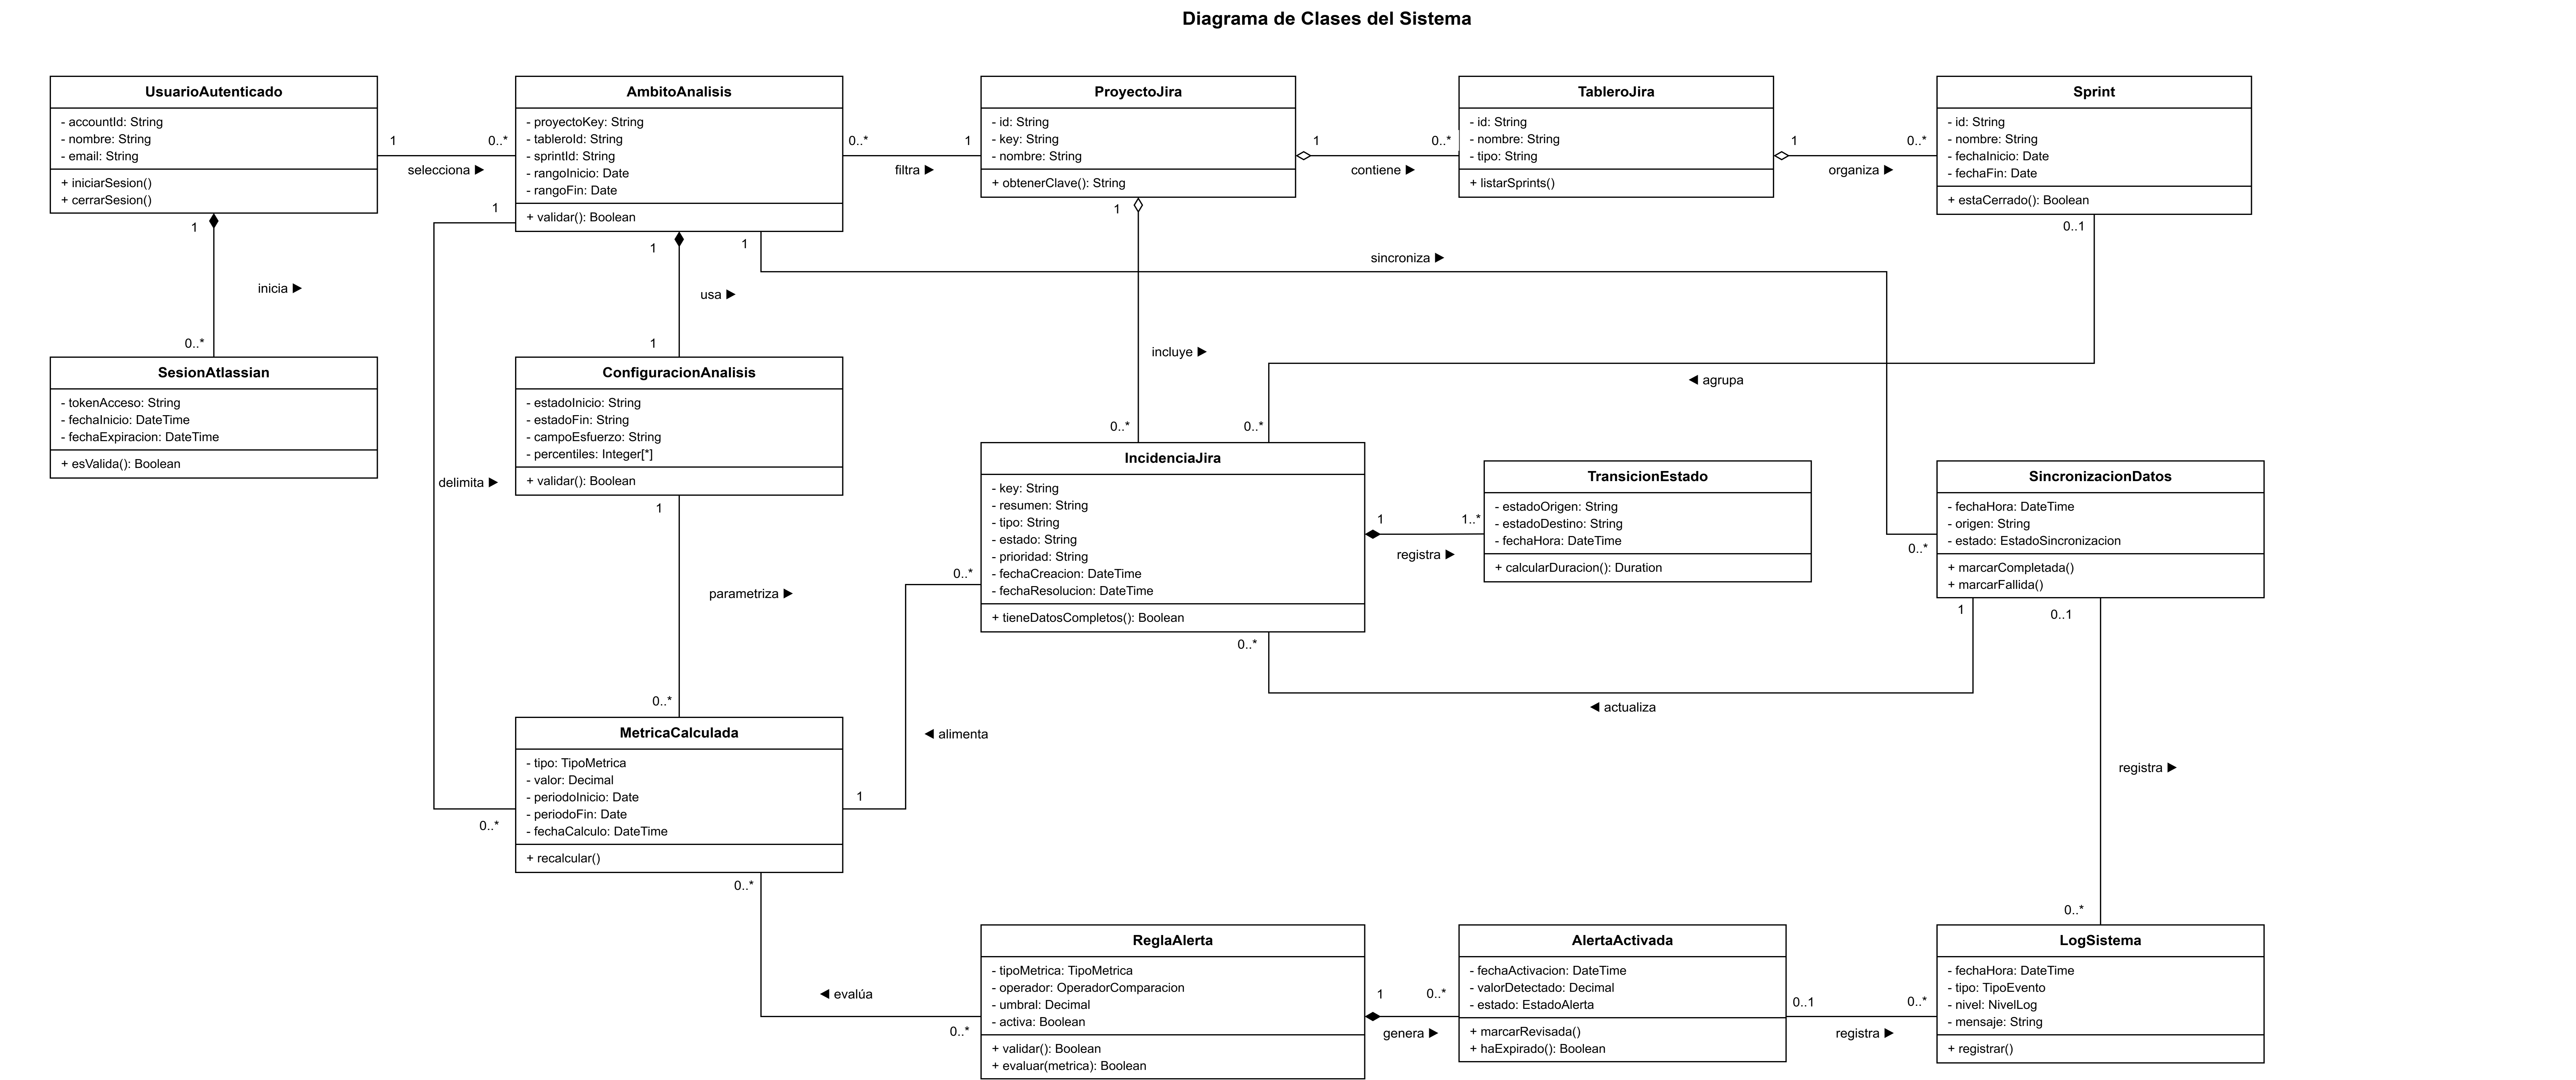
\includegraphics[width=1.12\linewidth,height=0.86\textheight,keepaspectratio]{diagrams/clases-dominio-sistema.png}%
    }
    \caption{Diagrama de clases del sistema}
    \label{fig:clases-dominio-sistema}
\end{figure}
\end{landscape}

La Figura~\ref{fig:clases-dominio-sistema} se interpreta a partir de los verbos situados sobre cada relación. El triángulo del verbo indica la dirección de lectura y las cardinalidades de los extremos concretan cuántas instancias pueden participar en cada asociación. En cuanto a la notación UML, según la especificación oficial de OMG \cite{OMGUML251}, el rombo blanco representa una agregación, es decir, una relación todo-parte débil en la que la parte puede existir de forma independiente. El rombo negro representa una composición, una relación todo-parte fuerte en la que la parte depende del ciclo de vida del todo.

Además de identificar las clases, es necesario indicar qué papel desempeña cada una dentro del dominio. La Tabla~\ref{tab:responsabilidades-clases} resume las responsabilidades principales y los atributos o conceptos más relevantes asociados a cada clase. Estos atributos no pretenden sustituir al diseño físico de la base de datos, sino aclarar qué información mínima necesita manejar el sistema para cumplir los casos de uso definidos.

\begin{landscape}
{\footnotesize
\begin{longtable}{>{\raggedright\arraybackslash}p{5.0cm}>{\raggedright\arraybackslash}p{8.0cm}>{\raggedright\arraybackslash}p{10.2cm}}
\caption{Responsabilidades y atributos principales de las clases del dominio}
\label{tab:responsabilidades-clases}\\
\toprule
\textbf{Clase} & \textbf{Responsabilidad principal} & \textbf{Atributos o información principal} \\
\midrule
\endfirsthead
\toprule
\textbf{Clase} & \textbf{Responsabilidad principal} & \textbf{Atributos o información principal} \\
\midrule
\endhead
\bottomrule
\endfoot
\texttt{UsuarioAutenticado} & Representar al usuario que accede a Nuvlo y delimitar la propiedad de sesiones, ámbitos de análisis y configuraciones. & Identificador interno, identificador de cuenta Atlassian, nombre visible, correo electrónico, fecha de alta, fecha de último acceso y estado de la cuenta. \\
\texttt{SesionAtlassian} & Mantener la información necesaria para operar en nombre del usuario autenticado sin pedir credenciales locales. & Identificador de sesión, usuario asociado, \textit{cloudId}, \textit{scopes} concedidos, fecha de creación, fecha de expiración y referencia segura a los \textit{tokens}. \\
\texttt{AmbitoAnalisis} & Definir el subconjunto de datos sobre el que se calculan métricas y se muestran resultados. & Nombre del ámbito, usuario propietario, proyectos incluidos, tablero o \textit{sprint} seleccionado, rango temporal, filtros activos y fecha de última sincronización. \\
\texttt{ConfiguracionAnalisis} & Recoger los criterios que modifican la interpretación de los datos y el cálculo de métricas. & Estados de inicio y fin, estados considerados trabajo en curso, campo de esfuerzo, percentiles visibles, agrupación temporal y criterios de exclusión. \\
\texttt{ProyectoJira} & Representar un proyecto importado desde Jira y servir como contenedor lógico de tableros e incidencias. & Clave del proyecto, nombre, identificador Jira, URL de origen, tipo de proyecto y fecha de última actualización local. \\
\texttt{TableroJira} & Modelar un tablero de trabajo de Jira asociado a un proyecto y usado para organizar la consulta de \textit{sprints}. & Identificador Jira del tablero, nombre, tipo de tablero, proyecto asociado y fecha de sincronización. \\
\texttt{Sprint} & Representar una iteración temporal utilizada para calcular \textit{Velocity} y analizar evolución por periodos. & Identificador Jira del \textit{sprint}, nombre, estado, fecha de inicio, fecha de fin, fecha de cierre y tablero asociado. \\
\texttt{IncidenciaJira} & Representar cada unidad de trabajo sincronizada desde Jira y aportar los datos base para métricas de flujo. & Clave, resumen, tipo, estado actual, prioridad, estimación, fecha de creación, fecha de resolución, proyecto asociado y responsable si está disponible. \\
\texttt{TransicionEstado} & Registrar los cambios de estado de una incidencia para reconstruir su recorrido y calcular tiempos. & Incidencia asociada, estado origen, estado destino, fecha de transición y origen de la información sincronizada. \\
\texttt{SincronizacionDatos} & Controlar cada proceso de actualización desde Jira o desde el conjunto de datos de demostración. & Ámbito afectado, instante de inicio y fin, estado de ejecución, número de elementos procesados, errores detectados y resumen del resultado. \\
\texttt{MetricaCalculada} & Almacenar el resultado de un cálculo de métrica para un ámbito, periodo y configuración concreta. & Tipo de métrica, valor agregado, periodo, percentiles, número de incidencias consideradas, fecha de cálculo y configuración utilizada. \\
\texttt{ReglaAlerta} & Definir condiciones configurables que permiten avisar al usuario ante valores relevantes de una métrica. & Métrica objetivo, operador, umbral, severidad, estado activo/inactivo, ámbito asociado y fecha de creación. \\
\texttt{AlertaActivada} & Representar una ocurrencia concreta generada cuando una regla cumple su condición. & Regla origen, métrica evaluada, valor observado, severidad, mensaje, fecha de activación y estado de revisión. \\
\texttt{LogSistema} & Conservar eventos relevantes para trazabilidad, depuración y explicación de operaciones internas. & Tipo de evento, severidad, mensaje, usuario o ámbito asociado, fecha de registro, origen del evento y fecha prevista de expiración. \\
\end{longtable}
}
\end{landscape}

A partir de estas responsabilidades se observa una separación entre clases de identidad y configuración, clases procedentes del dominio Jira, clases de cálculo y clases de trazabilidad. Esta división facilita que el sistema pueda sincronizar información externa, conservar una representación local estable y calcular métricas sin depender de una llamada directa a Jira en cada consulta del usuario.

\clearpage
\section{Diagrama entidad-relación de la base de datos}

El diagrama entidad-relación describe la estructura lógica prevista para la persistencia del sistema. A diferencia del diagrama de clases, que representa conceptos del dominio y responsabilidades de análisis, este modelo se centra en tablas, claves primarias, claves foráneas y cardinalidades. Para facilitar su lectura se emplean entidades rectangulares con sus atributos internos y relaciones representadas mediante rombos, siguiendo la forma habitual de los diagramas entidad-relación y las formas disponibles en draw.io para modelos de bases de datos~\cite{DrawioERTables}. Cada rombo contiene un verbo que describe la relación y las cardinalidades se sitúan junto a los extremos conectados. Los nombres de tablas y columnas se han planteado en minúsculas y con \texttt{snake\_case}, siguiendo criterios habituales de estilo SQL~\cite{HolywellSQLStyle}; además, se evitan estructuras innecesariamente complejas para mantener un diseño comprensible y normalizado, de acuerdo con las recomendaciones generales de diseño relacional recogidas por Karwin~\cite{Karwin2010SQLAntipatterns}.

\begin{figure}[htbp]
    \centering
    \makebox[\textwidth][c]{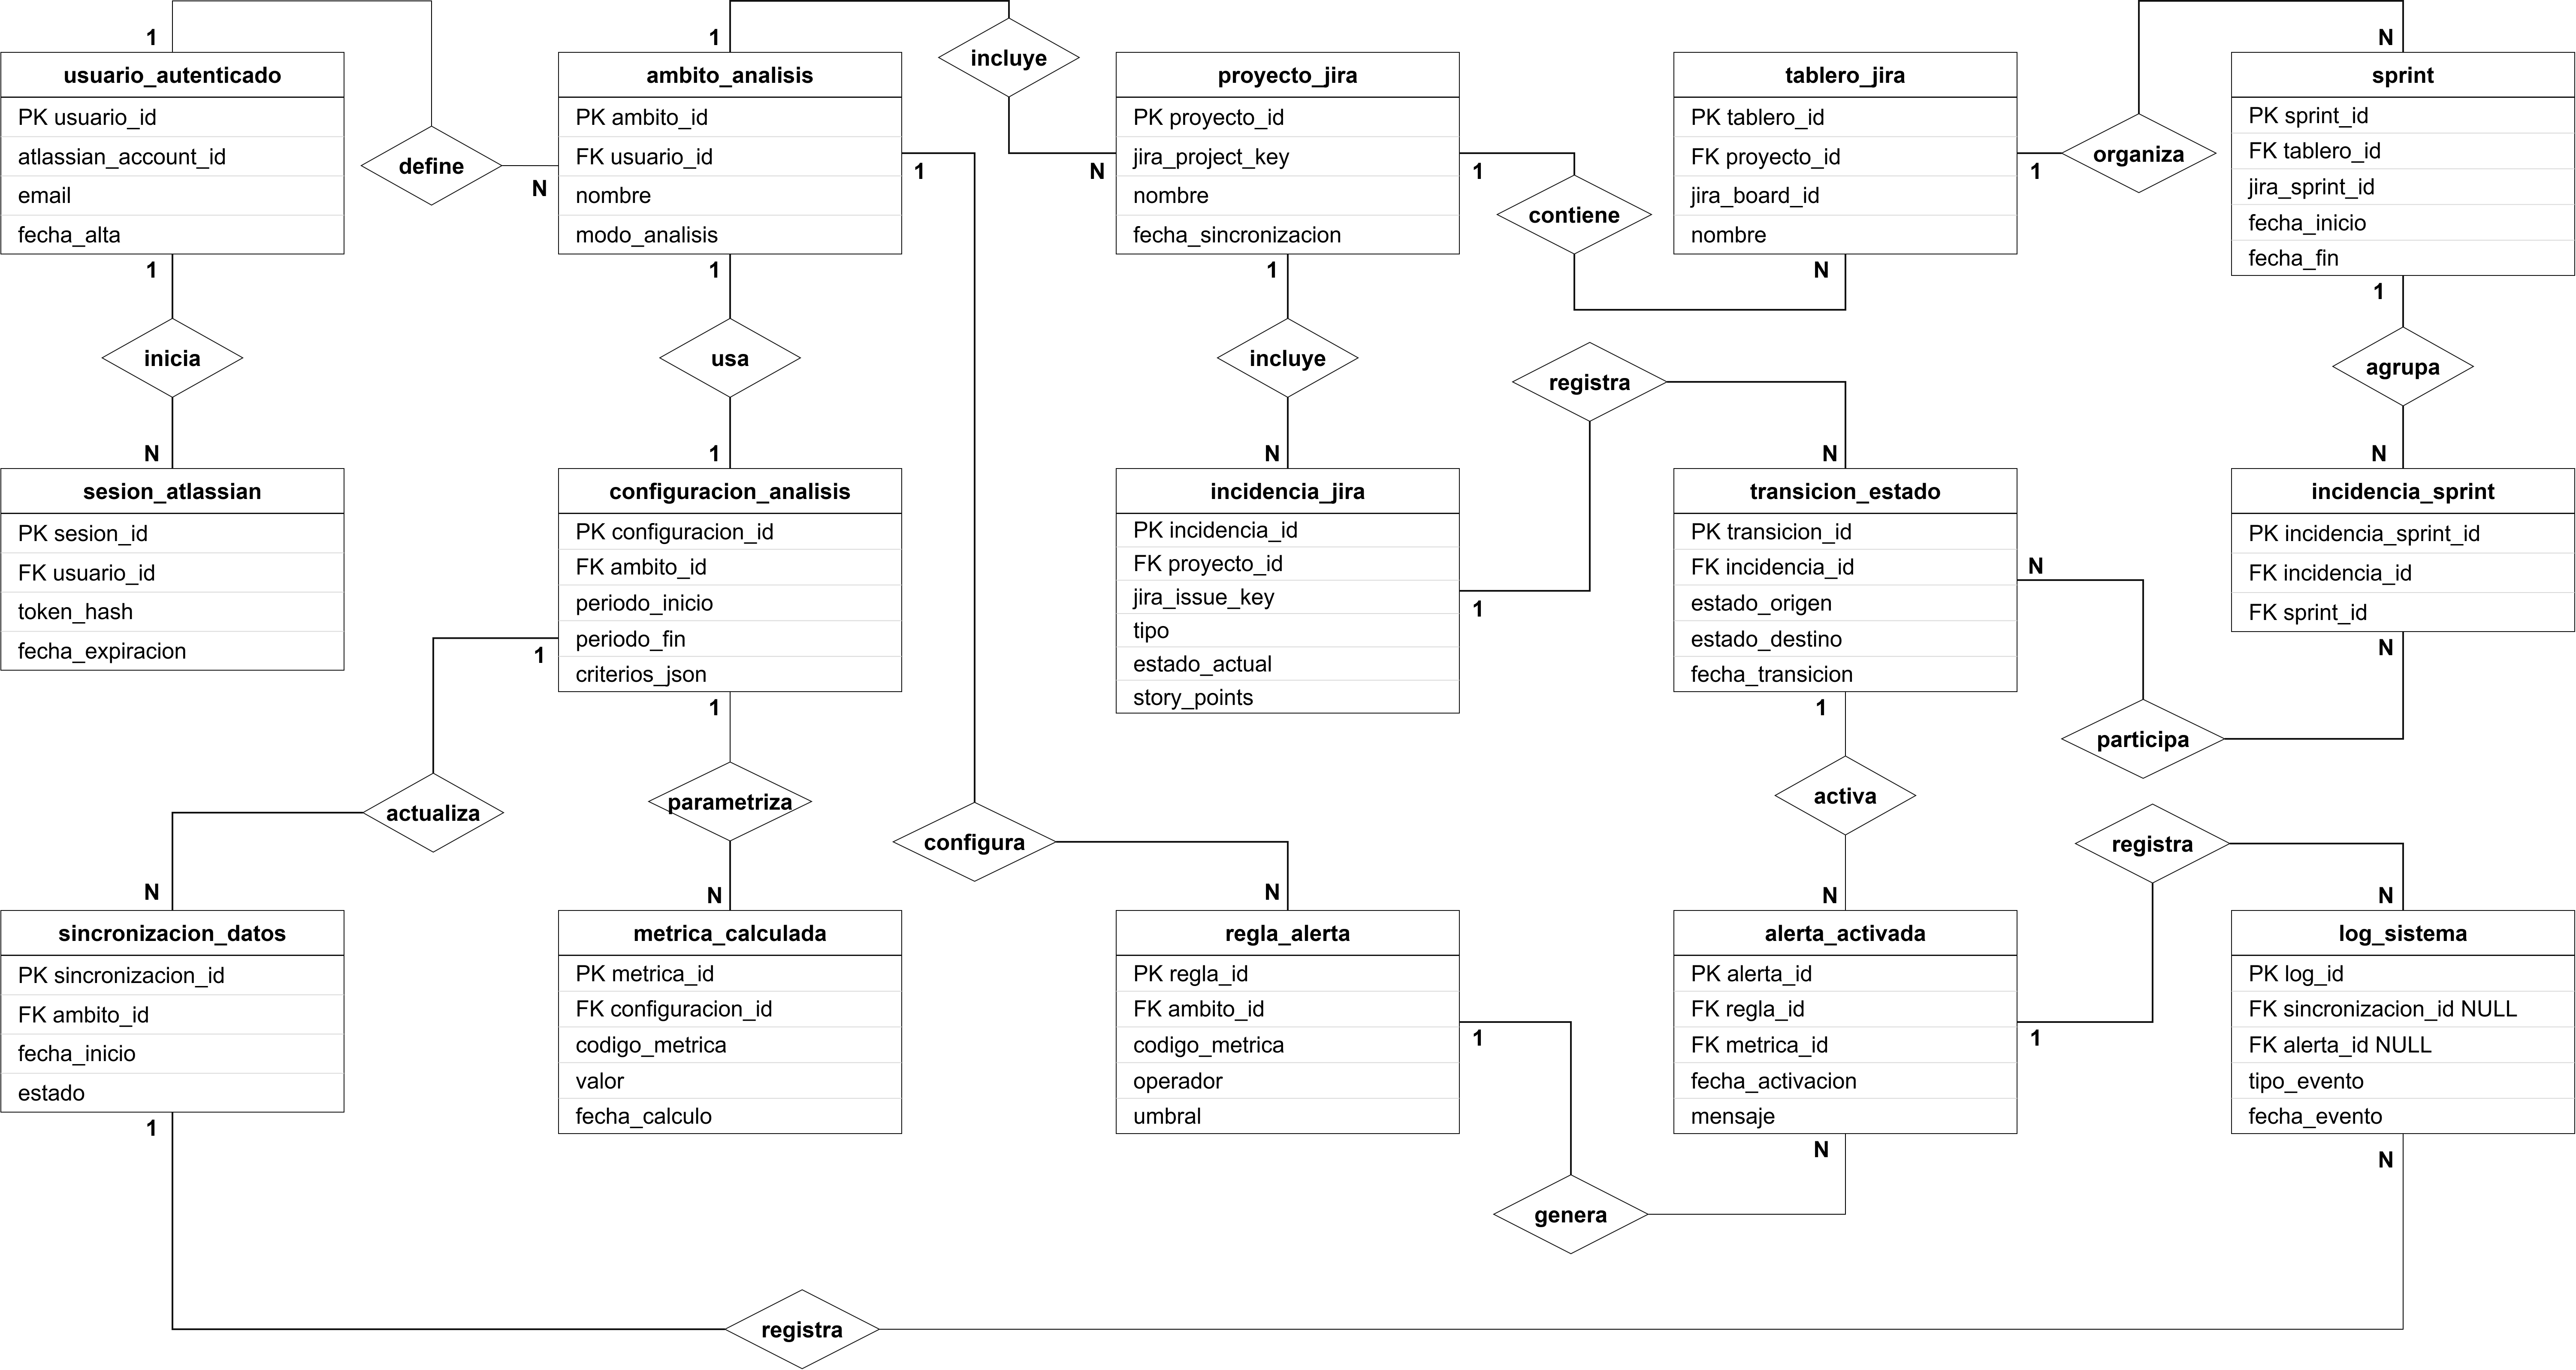
\includegraphics[width=1.25\textwidth]{diagrams/entidad-relacion-base-datos.png}}
    \caption{Diagrama entidad-relación de la base de datos}
    \label{fig:entidad-relacion-base-datos}
\end{figure}

La Figura~\ref{fig:entidad-relacion-base-datos} toma como referencia las entidades principales del diagrama de clases, pero las adapta a un modelo persistente. Las tablas puente \texttt{ambito\_proyecto} e \texttt{incidencia\_sprint} permiten resolver relaciones de muchos a muchos sin duplicar información ni forzar dependencias artificiales.

\begin{itemize}
    \item \texttt{usuario\_autenticado}, \texttt{sesion\_atlassian}, \texttt{ambito\_analisis} y \texttt{configuracion\_analisis}: almacenan la información del usuario, sus sesiones de Atlassian y los criterios de análisis definidos para cada ámbito. Un usuario puede iniciar varias sesiones y definir varios ámbitos; cada ámbito mantiene una configuración de análisis.
    \item \texttt{proyecto\_jira}, \texttt{tablero\_jira}, \texttt{sprint}, \texttt{incidencia\_jira} y \texttt{transicion\_estado}: representan los datos sincronizados desde Jira. Un proyecto puede contener varios tableros e incidencias, un tablero organiza \textit{sprints} y una incidencia registra sus transiciones de estado para calcular métricas de flujo.
    \item \texttt{ambito\_proyecto} e \texttt{incidencia\_sprint}: actúan como tablas intermedias. La primera asocia ámbitos de análisis con proyectos Jira; la segunda relaciona incidencias con \textit{sprints}, evitando una relación directa rígida cuando una incidencia pueda aparecer en más de una iteración.
    \item \texttt{sincronizacion\_datos}, \texttt{metrica\_calculada}, \texttt{regla\_alerta}, \texttt{alerta\_activada} y \texttt{log\_sistema}: guardan la actividad interna del sistema. Las sincronizaciones actualizan un ámbito, las métricas se calculan a partir de la configuración vigente, las reglas evalúan dichas métricas y las alertas y \textit{logs} conservan la trazabilidad del funcionamiento.
\end{itemize}
\clearpage
